\documentclass{article}

%%%%%%%%%%%%%%%%%%%%%%%% Importation de paquets %%%%%%%%%%%%%%%%%%%%
\usepackage{polyglossia}
\usepackage{graphics}
\usepackage{fontspec}
\usepackage{fancyhdr}
\usepackage{listings}
\usepackage{graphics}
\usepackage{fancyhdr}
\usepackage{vmargin}
\usepackage{epsfig}   
\usepackage{multicol}
\usepackage{multirow}
\usepackage{url,hyperref}

%%%%%%%%%%%%%%%%%%%%%%%% Format, langue, marges %%%%%%%%%%%%%%%%%%%%%%%%%%

\setdefaultlanguage{english}
\defaultfontfeatures{Mapping=tex-text,Scale=MatchLowercase}
\setmainfont{Linux Libertine O}
\setpapersize{A4}
\setmarginsrb   
{35mm}  % leftmargin
{20mm}  % topmargin
{35mm}  % rightmargin
{40mm}  % bottommargin
{14pt}  % headheight
{15mm}   % headsep
{20pt}  % footheight
{20mm}  % footskip

%%%%%%%%%%%%%%%%%%%%%%%% En-tete et pied de page %%%%%%%%%%%%%%%%%%%%%%%%%%
\pagestyle{fancy}
\fancyhf{}
\lhead{\scalebox{0.1}[0.1]{
\includegraphics{./Images/enseeiht}}}
\rhead{\scalebox{0.1}[0.1]{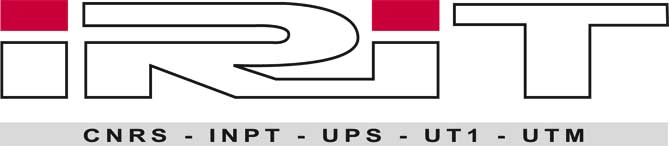
\includegraphics{./Images/irit}}
\lfoot{Three-dimensional modeling and printing}}
\rfoot{\bfseries \thepage}

\begin{document}

\bigskip
\bigskip
\bigskip
\bigskip
\bigskip
\bigskip
\bigskip
\bigskip

\begin{center}
\LARGE{Three-dimensional modelling and printing project :\\User documentation \\}
\bigskip
\bigskip\begin{tiny}
\end{tiny}
\Large{from January 23 to March 16, 2012}
\end{center}

\bigskip
\bigskip

\begin{center}
\large{
\textit{Vincent \textsc{Duvert} \\
Antoine \textsc{Lubineau} \\
Caroline \textsc{Naud} \\
James \textsc{Packer} \\
Florian \textsc{Ribon}} \\
\bigskip
INP-ENSEEIHT/IMA 
}
\end{center}

\bigskip
\bigskip

	This report summarizes the context, organization, work and outcomes within the project 3D modeling and printing project suggested by the VORTEX team of IRIT to some of the third-year students in the IMA department of ENSEEIHT.

\bigskip
\bigskip

\begin{figure}[!h]
\begin{center}
\scalebox{0.4}[0.4]{
\includegraphics{./Images/enseeiht}}
\end{center}
\end{figure}

\bigskip

\begin{center}
http://www.enseeiht.fr/fr/index.html \\
2 Rue Charles Camichel \\
31 071 TOULOUSE
\end{center}

\bigskip

\begin{figure}[!h]
\begin{center}
\scalebox{0.4}[0.4]{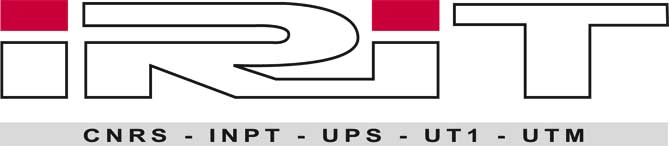
\includegraphics{./Images/irit}}
\end{center}
\end{figure}

\begin{center}
http://www.info@irit.fr\\
Université Paul Sabatier \\
118 Route de Narbonne \\
F-31062 TOULOUSE CEDEX 9
\end{center}

\thispagestyle{empty}

\newpage

\tableofcontents

\newpage

\section{Reminding of the global architecture of the application}


\begin{figure}[!h]
\begin{center}
\scalebox{0.4}[0.4]{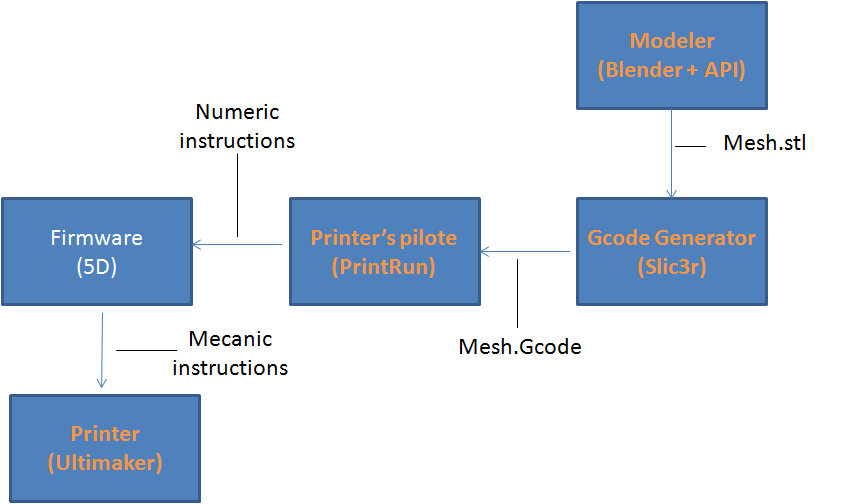
\includegraphics{./Images/ARD1}}
\end{center}
\end{figure}

\newpage

\section{The modeling part on Blender}

\subsection{Point on the graphic interface}

Blender's graphic user interface remains quite difficult to use for inexperienced users and shows ``useless'' functions for users only aiming at modeling, correcting meshes and printing them. In Blender, the user has the possibility to manually modify this graphic interface as he wants to only keep the most useful features visible. That's what was done in that case and the first view available when starting Blender will be this one : 
\bigskip
\bigskip

\begin{figure}[!h]
\begin{center}
	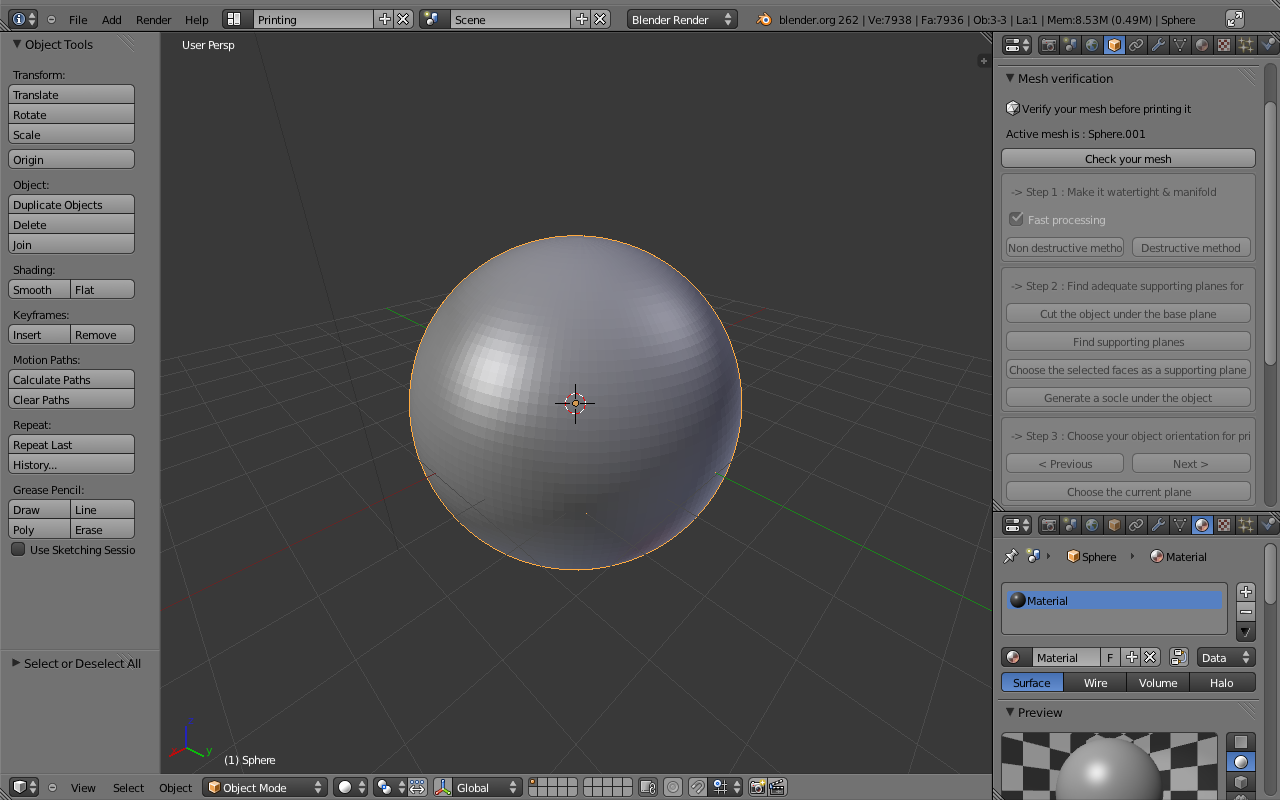
\includegraphics[scale=0.3]{./Images/NotreInterface}
\end{center}
\end{figure}

\bigskip
\bigskip

We only chose to keep visible what was necessary to a user simply wanting to import, modify and correct a mesh but you can create as many configurations as you want by simply drag and dropping some windows and panels and registering the corresponding file (\textit{startup.blend}) thanks to a simple Ctrl + U.\\

The part we see at the right of the screen below and which seems a little grey is the panel we added so that the user can have access to the different functions we implemented. It is visible next page.

\newpage

\bigskip
\begin{figure}[!h]
\begin{center}
	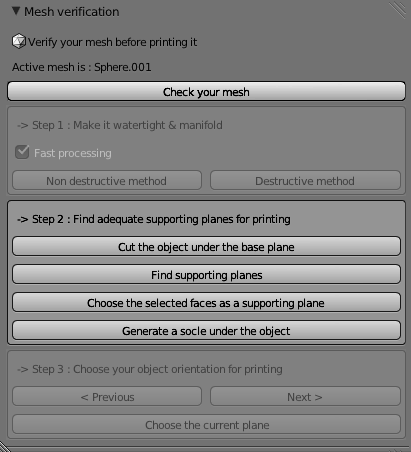
\includegraphics[scale=0.8]{./Images/Panel}
\end{center}
\end{figure}
\bigskip

As for the organization of the Mesh Verification panel, it is devided into 4 main parts called ``steps'' since the user has to use them successively. We detail these steps here below.\\

\textbf{Step 0 : not written on the panel} \\

This part of the panel reminds the user of the active mesh in the scene. It is also the first and only enabled button in the panel when starting Blender. It is to be used when the mesh is satisfying for the user to check if it is correct or not (manifold and watertight). By passing the mouse over the button, a description of the action is given, as for all the buttons and check boxes. When pressing this ``Check your mesh'' button, the script of verification will be run and its outcome will determine the next step enabled. If the mesh is found incorrect, the user will see the first step enabled and only this step. If it is found correct, the second step will be enabled.\\

\textbf{Step 1 : the mesh correction step} \\

This step enables a check box and two different buttons allowing the user to correct the mesh the way he wants and in a chosen time (see the buttons description). When the mesh is considered correct by the script run when pressing the buttons, the step 2 is enabled. 

\newpage

\textbf{Step 2 : the finding of an adequate supporting plane for printing}\\

This step has been realized so that the user can both trust the application to find an adequate supporting plane for his object and decide of the supporting plane himself. \\

This last possibility is included in the ``Cut the object under the base plane'' button. This button allows the user to plane his object himself where he wants be orienting it and positioning it considering the $z = 0$ plan. This can be useful when printing an egg for example. In this case, there is no plane to support the object. Another button enabling the user to choose the supporting plan himself is the third one when he can select one and choose it so that the object will be automatically oriented as chosen.\\

But in this step, the user can also trust the scripts implemented to find several adequate supporting planes on the object (the number of planes generated being chosen by the developer). When this button is pressed, the ``best'' plane found according to the script is highlighted and the third step is enabled to choose between all the other planes.\\

\textbf{Step 3 : the choice between the generated planes}\\ 

In this step, planes have previously been found to support the object and the ``Next'' and ``Previous'' buttons allow the user to navigate among them, highlight them and select one for supporting the object. Once the ``Choose the current plane'' button is pressed, the step 0 is enabled again while the third one is disabled. 

\subsection{Obtaining an object}

\subsubsection{Loading an existing mesh from a file}

You can simply import an object into Blender, preferably from a PLY or STL format. Many printable objects are findable with simple online resarches like in \href{http://graphics.stanford.edu/data/3Dscanrep/}{the Stanford 3D models repository}, or import any other 3D object and use our tools to repair their meshes and make them fully ready for print.
To import an object, simply open Blender then open the File menu and click on "Import".

\subsubsection{Creating and editing your own mesh}

To build your own object from sratch, you can use all standard Blender functionnality. You may want to read some Blender documentation, but if you want to quickly make a simple printable object, the best way is to start by adding to the scene some primary meshes ('Add' menu, then chose a mesh like a Cube or a Cylinder), place them wherever you want, then you may edit your meshes, Blender offering two main ways to do it. The first one consists of vertex per vertex and precise edition (Edit Mode), and the second one allows you to manipulate areas of vertices in a smoother way (Sculpt Mode). Finally you have to merge them into a single object if you want to make it printable. To do that, right click on any of your mesh, then look for the modifiers into the right panel and add a Boolean - Union one with any other object. Now you can remove your second object as the first one is a result of the union.

\subsection{Verifying and repairing your mesh}

To be printable, your mesh have to be watertight and manifold. To know if it is the case, simply click on the 'Check your mesh' button on our customized UI. If the UI goes directly to step 2 without enabling the step 1 buttons, then all is OK and the mesh is correct. If not, you can easily correct your mesh with two different ways. If your object is not very damaged or doesn't contains many edges, try the non destructive method. But if you want to be sure that the resulting object is perfect, you may click on the destructive method. Besides, checking the fast-processing option should improve a lot the speed of the algorithm process, but may result in unwanted artifacts. Anyway, you can cancel your previous commands with CTRL+Z and try again with differents options.

\subsection{Generating adequate supporting plans for your object}

\subsection{Choosing and applying a good supporting plan}

\subsection{Saving and exporting your mesh}

Once your object has a correct mesh and is well oriented, you simply have to export it. Open the 'File' menu and click on 'Export' with the STL format. Your resulting STL file is now ready to be sliced and printed !

\newpage

\section{The printing part}

\subsection{Preparing the Utimaker 3D printer}

It usually takes a bit of time to get a nice consistant extrusion at the beggining of the print, to avoid that put a few perimeters of skirt in Slic3r and push a bit on the filament during the first few seconds.
It is also a good idea to regularly check that the screw pushing on the filament stays nice and tight and that the roll of filament doesn't get caught and stops turning.

\subsection{Generating the GCode on Slic3r}

First read \href{http://richrap.blogspot.com/2012/01/slic3r-is-nicer-part-1-settings-and.html}{this wiki} about the meaning of most the parameters. \\

And here are some useful values we found out worked fairly well in most cases :
\begin{itemize}
\item \textbf{Temperature} : A good value is usually between 220 and 240. Lower and the plastic has difficulties sticking to the board at the beginning, higher and it might not cool down fast enough between layers. A high temperature also decreases the pressure the extruder has to apply
\item \textbf{Extrusion multiplier} : Because of difference in the way Slic3r and the arduino measure the length of filament to extrude (one measures it at the nozzle while to other does it at the motor) you have to multiply the theoritical value by a coefficient between 150 and 180.
\item \textbf{Print speed} : these five parameters depend mostly of the object's size. Indeed for most objects (30-30-60-60-60) are good value as they will insure a good quality and a good speed. However for small objects going too fast will not allow for enough time the layers to cool down and so the print will be less precise. The most 0.7 version of Slic"r corrects that bug by automatically slowing down when a layer is too small to cool down fast enough otherwise.
\item \textbf{Layer height} : The evident idea here is that a smaller layer height will make for a better quality. The values should be between 0.2 and 0.4 mm, however while 0.2 mm provides a very nice quality print it makes it longer and sometimes the plastic will bend more easily while cooling down.
\item \textbf{Skirt} : adding more loops before the actual print gives you a bit more time to make sur the extrusion is good.
\item \textbf{Retraction} : the values influence what the printer will do in case of a bridge (jumping from a position to another without extruding). Playing
\end{itemize}

There other settings were tested that don't necessarily have an impact on the quality of the print but that are useful for other reasons.
\begin{itemize}
\item \textbf{Center} : sets the center of the object you're going to print, the center of the plate is (100,100).
\item \textbf{Copies along X/Y} : very useful to do numerous copies of small objects.
\item \textbf{Perimeters} : can be played wth in the case of thin walled objects.
\item \textbf{Infilling} : the fastest to calculate is rectilinear but in some cases concentric is much more sensible (for instance, when most layer are homeomorphic to a circle.
\end{itemize}

\subsection{Sending the instructions to the printer with PrintRun}
All needs to be done now is to send the G-code and the M-code to the printer via printrun. Some errors we're detected in that area like checksum mismatch erros mostly due to problems with the USB port. The only actions that can be done while printing are :
\begin{itemize}
\item Check the temperature of the nozzle.
\item Set the temperature.
\item Pause the print, and then resume or restart.
\end{itemize}


\end{document}
